% Generated by thesis/ch7/exp1/churn_case_figures.py -- do not edit by hand.
\begin{figure}[tbp]
  \centering
  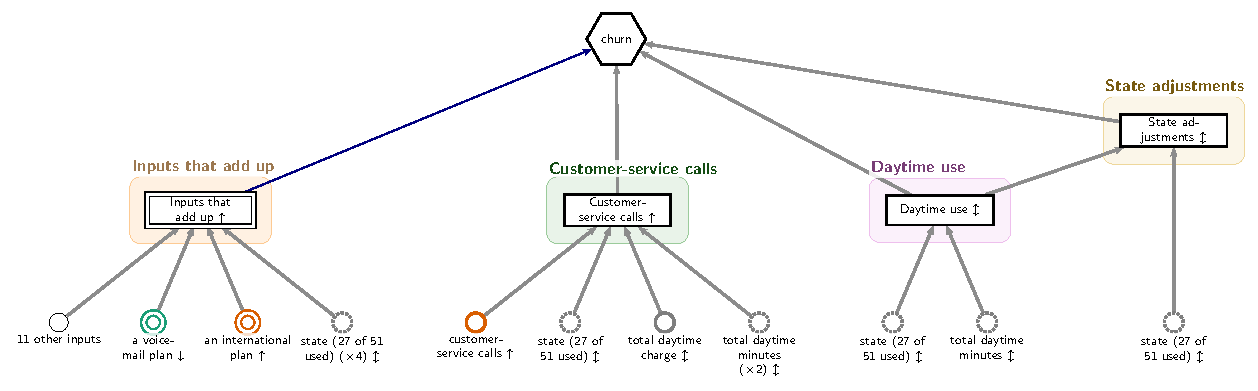
\includegraphics[width=\textwidth,height=0.8\textheight,keepaspectratio]{figures/ch7/churn-case-net-concept.pdf}
  \caption{Churn case network (seed 10) at the level of its parts. Each top-level part of the explanation is one box, with the inputs it reads below it and the churn score at the top. Arrows on inputs and boxes: the direction of the effect on the final prediction (up raises it, down lowers it, double arrow depends). Edges: blue, a positive weight (raises the score); red, a negative weight; thicker, a larger weight; grey, no single weight (the inputs a collapsed part reads, and a part's sum). Double outline: acts at a fixed rate everywhere (dashed double: on the observed data). A grouped input (state) stands for its used levels; \emph{11 other inputs}: the rest of the inputs of \emph{Inputs that add up}.}
  \label{fig:ch7-churn-case-net-concept}
\end{figure}
